%!TEX root = ../lectures_olympics.tex

\chapter{电磁场理论,电磁波}
至此我们已经学过了电磁场理论的主要部分,明白了电荷产生电场、电流,也就是运动的电荷产生磁场,与此同时电磁感应定律先诉我们,不但电荷会产生电场,变化的磁场同样可以产生电场等电磁场的基本规律。
但当将这些实验现象和已知规律放在一起的时候,会导致一些意想不到的结果。
经过充分的思考,麦克斯韦(\textit{J. C. Maxwell})在电磁场方程中加入了一项,成功地解决了这些矛盾,和之前的理论一起构成了近代电磁理论的基石,麦克斯韦也成了电磁理论的奠基人,描写电磁场运动的方程则被后人称为{\heiti 麦克斯韦方程组}(Maxwell's Equations)。

\section{麦克斯韦的电磁场理论}


如图\ref{fig:em-theory-1}所示均匀的具有弱导电性的介质中一点有一些电荷$Q$,随着时间的推移这些电量逐渐地流出。
根据对称性可知电流密度成球对称分布,考虑如图所示所回路$\Gamma$,在它内部有向外的电流$j$,根据安培环路定理,理应有磁场的存在,并且有图中箭头方向。
可是另一方面,在一个球对称的球面上根据对称性的分析,是不可能存在图中所示的磁场的,不同回路的选取会得到对磁场方向完全不同的结论。
这预示着电磁场理论有不完整之处,需要对其进行扩充。

\begin{figure}
\setcaptionwidth{0.45\textwidth}
\begin{minipage}[t]{0.5\linewidth}
\centering

\includegraphics[width=0.8\textwidth]{images/em-theory-1.pdf}
\caption{径向分布的电流,通过安培环路定理无法给出正确的磁场分布}
\label{fig:em-theory-1}
\end{minipage}%
\begin{minipage}[t]{0.5\linewidth}
\begin{flushright}
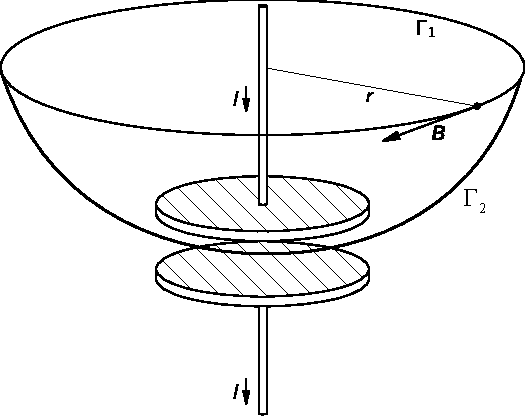
\includegraphics[width=0.8\textwidth]{images/em-theory-2.pdf}
\caption{对正在充电的电容在不同的回路上应用安培环路定理得到不同的结果}
\label{fig: em-theory-2}
\end{flushright}


\end{minipage}
\end{figure}




另外一个著名的例子来自于一个正在充电的电容器。
如图\ref{fig: em-theory-2}所示有一个电容正在被充电,导线中的电流为$I$,在环路$\Gamma_1$上应用安培环路定理,距离导线$r$处的磁感应强度应为
\begin{equation}
B = \frac{\mu_0I}{2\pi r}.
\end{equation}
但是安培环路定理并不仅限于像$\Gamma_1$那样的规则环路,而是对任意形状的回路和表面均成立,考虑图中的回路$\Gamma_2$,按道理说它应该得到相同的磁感应强度,但是由于环路以及表面上并没有电流通过,所以安培定律将得到磁感应强度为零这样错误的结论。


类似的推理还有很多,它们无一例外地表明,前面的电磁理论依然不完整,需要加入新的内容。
而且看上去前面两个问题均与处于变化状态的电场有关,第一个问题由于电流的流出,每个闭合球面内的电荷不断减少,根据高斯定律电场强度也不断变化;第二个问题中处于充电状态的电容器内两板之间的电场强度也在不断地变化。
麦克斯韦认为,不仅是真实运动的电荷产生的电流会产生磁场,与此同时当电场强度发生变化时,也有相应的磁效应,看上去和电流产生磁场的效果没有什么不同,他将由电场强度的变化产生磁场产效应称为{\heiti 位移电流}(displacement current),这样安培环路定理在考虑了位移电流效应以后变成了
\begin{equation}
\int_L \vec{B}\cdot d\vec{l} = \mu_0\int_S \vec{j}\cdot d\vec{S} + \mu_0\varepsilon_0\frac{d}{d t }\int_S \vec{E}\cdot d\vec{S}.
\end{equation}
这样完整的电磁理论就被建立了出来。

下面我们来总结一下经典的电磁理论所包含的所有内容。
当空间中存在有电场、磁场和带电粒子时,电场、磁场的值以及它们随时间的变化关系由电荷、电流以及电磁场本身所决定。
定义两个矢量场$\vec{E}(x,y,z,t)$和$\vec{B}(x,y,z,t)$分别代表空间中各点在各个时刻电场强度和磁感应强度,它们在不同位置上有不同的值,并且有可能随时间而变化。
当带电粒子的位置和速度为已知时,用电荷密度$\rho(x,y,z,t)$和电流密度$\vec{j}(x,y,z,t)$来描写。
这样电磁场理论由以下三个部分构成:
\begin{description}
\item[{\heiti 麦克斯韦方程组}(Maxwell's Equations)]

电场、磁场的变化满足麦克斯韦方程组,由两个矢量方程和两个标量方程构成:
\begin{eqnarray}
\oint_S \vec{E}\cdot d\vec{S}&=& \frac{1}{\varepsilon_0}\int_V \rho dV\label{eqn: maxwell-equation-1}\\
\oint_L \vec{E}\cdot d\vec{l}&=& -\frac{d}{dt}\int_S \vec{B}\cdot d\vec{S}\label{eqn: maxwell-equation-2}\\
\oint_S \vec{B}\cdot d\vec{S}&=&\label{eqn: maxwell-equation-3} 0\\
\oint_L \vec{B}\cdot d\vec{l}& =& \mu_0\int_S \vec{j}\cdot d\vec{S} + \mu_0\varepsilon_0\frac{d}{d t }\int_S \vec{E}\cdot d\vec{S}\label{eqn: maxwell-equation-4}
\end{eqnarray}
以上的方程称为麦克斯韦方程的积分形式。

第一个方程\ref{eqn: maxwell-equation-1}是{\heiti 电高斯定理},它告诉我们,对于任何一个闭合曲面,电场线的面积分,也就是熟知的电通量正比于曲线内部所包围的总电荷,实践表明高斯定律不但对于静电场,对于任意变化的电磁场和运动的电荷也同样是成立的。

第二方程\ref{eqn: maxwell-equation-2}则是熟知的{\heiti 法拉第电磁感应定律},或者称为{\heiti 电环路定理}它表明沿着任意闭合回路电场强度的线积分,也就是电动势等于穿过以曲线为边界任意一个曲面的磁通量随时间的变化率。
它并没有告诉我们比电磁感应定律更多的内容,但是需要注意的是闭合回路本身也是可以运动的,另外注意正方向的选取。

第三个方程\ref{eqn: maxwell-equation-3}是{\heiti 磁高斯定理},它指出,对于任意闭合曲面的磁通量必然为零,也就是说自然界不存在孤立的磁单极子,无论带电体或磁铁的运动状态如何均无法将磁荷分离。

最后一个方程\ref{eqn: maxwell-equation-4}则是由麦克斯韦扩充了的{\heiti 安培环路定律},即{\heiti 磁环路定理}。它告诉我们不但电流、变化的电场也会形成相应的磁场。
正是由于变化的电场会引起磁场,再加上方程\ref{eqn: maxwell-equation-2}给出的变化的磁场引起电场,两个现象共同导致了不断变化的电磁效应会不断地向外传递,从而形成了电磁波。

\item[{\heiti 洛伦兹力公式}(Lorentz Force Equation)]
当电荷为$q$,速度为$\vec{v}$的带电粒子在电磁场中运动时,它的受力为电场力和磁场力的合力,这种情况下把这个合力(而不单是磁场力)称为洛伦兹力:
\begin{equation}
\vec{f} = q\vec{E}+q\vec{v}\times\vec{B}.
\end{equation}\label{eqn: 洛伦兹力}
如果说麦克斯韦方程组给出了电荷和电流如何影响电磁场的话,这里给出的就是在给定的电磁场中运动的电荷是如何受电磁场作用的。
无论是电场力还是磁场力过去都已经讨论了很多,这里需要注意的就是如果带电粒子本身的电磁效应对现有的电磁场分布影响较小时,带电粒子的运动不会影响电磁场的分布,这时计算相对简单。
但很多问题当中带电粒子不但在电磁力作用下运动,而且它们同时也是贡献电磁场的主要因素时,问题将会变得极其复杂。
\item[{\heiti 电荷守恒}(Conservation Law of Electric Charge)]
带电粒子的电荷在运动与相互作用过程中代数和保持不变\footnote{若电荷做低能的,非相对论的运动则既不会凭空产生也不会凭空消失。然而高能相对论性的电磁相互作用将导致电荷的产生与湮灭,比如正负电子对湮灭为两个光子:$e^- \,\, + e^+ \longrightarrow 2\gamma$。即使在这样的过程中正负电荷代数和也是守恒的。}
\begin{equation}
\frac{d}{dt}\int_V\rho dV+\int_S \vec{j}\cdot d\vec{S} = 0.
 \end{equation}
这是自然界中最基本、最严格的守恒定律之一,从某种意义上讲它规定了电磁相互作用理论应有的形式。
任何一个闭合曲面内电量的减少一定与它表面上的电流有联系,而上式则定量地给出了这种联系。
从某种意义上讲,位移电流引入的目的也是为了使电磁场定律与电荷守恒相容,感兴趣的同学可以通过阅读和计算发现这一点。



\end{description}



%%%%%%%%%%%%%%%%%
\begin{example}
你能否证明,在引入位移电流以后能够解释图\ref{fig:em-theory-1}和图\ref{fig: em-theory-2}出现的悖论。
\tagged{student}{\vspace*{4cm}}
\begin{taggedblock}{teacher}
\noindent
解析:引入位移电流以后,第一种情况下真实的电流完全被位移电流所抵消,所以没有磁场。

第二种情况下给电容充电过程中电场会产生变化,通过计算可以表明电场的变化率对磁场的贡献刚好与电流完全相等,所以可以避免错误的结果。
\end{taggedblock}
\end{example}
%%%%%%%%%%%%%%%%%%%%%%




\section{电磁波}

正是因为变化的磁场能够产生涡旋电场、而变化的电场又会引起位移电流,这样在电磁场的交替感应下当空间当中一点处的电磁场发生剧烈变化,例如一个带电粒子在做往复振动时,它引起的电磁场就会在电磁场自身的相互作用下将变化的效果向外传递,从而形成了{\heiti 电磁波}(electromagnetic wave)。
完整地研究电磁波的性质和特点远远超出我们目前的能力范围,这里将在简单的情况下了解电磁波的特点和一些定性的结论,严格的数学计算留给同学们课后研究。

做为一种波动现象,电磁波和普通的机械波有相似之处,也有本质的不同。
它们之间的相似性更多地体现在数学层面,对电磁波和机械波的描写有着相似的物理量。
例如振幅、波长、频率、周期和相位等等,对于简单的平面波来说,电磁波所携带的能量也正比于振幅的平方,其波长、频率和波速之间也满足
\begin{equation}
c = \lambda\nu
\end{equation}
其中$c$为电磁波的波速,后面我们将看到它正是熟悉的光速,$\lambda$、$\nu$分别为电磁波的波长和频率。
与机械波的一个重要的不同是电磁波的传播并不需要介质,在真空中也能够传播;这一点和声波(一种典型的机械波)是很不同的,我们知道在地球以外的太空中,由于没有介质所以声音无法传播。
另外机械波依据振动和波的传播方向的不同有横波和纵波之分,但电磁波无一例外均为横波。
这样根据三维空间的特性,一列沿直线传递的平面电磁波有两个独立的振动方向。

\begin{figure}[htb]
\centering
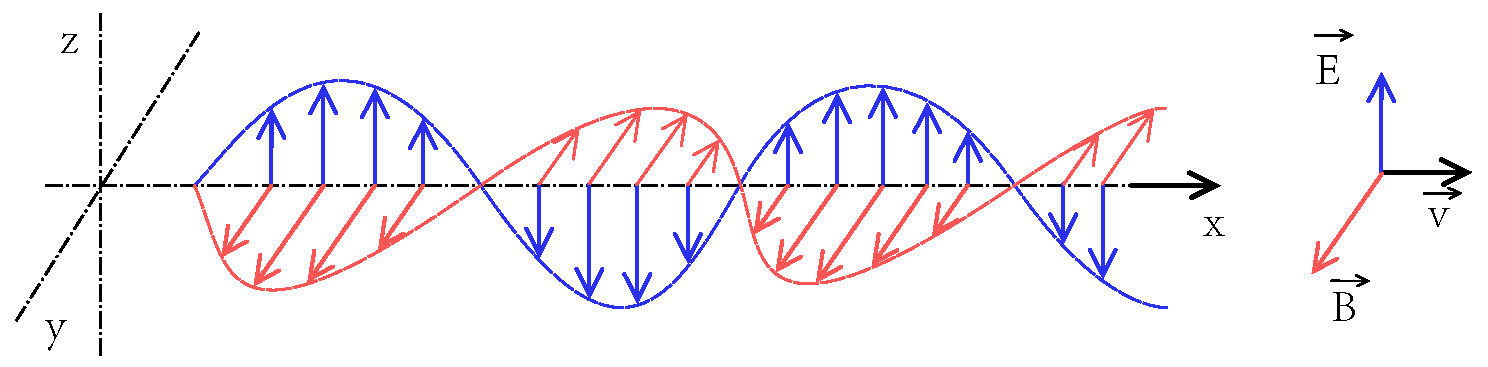
\includegraphics[width=0.7\textwidth]{images/em-theory-5.pdf}
\caption{平面电磁波,电、磁场均垂直于传播方向且彼此垂直}
\label{fig: em-theory-5}
\end{figure}

根据麦克斯韦的电磁理论,真空中电磁波传播的波速并不是一个独立的物理量,而是由静电学和静磁学中两个基本量:真空介电常数$\varepsilon_0$和真空的磁导率$\mu_0$共同决定:
\begin{equation}
c = \frac{1}{\sqrt{\varepsilon_0\mu_0}} = 299792458\unit{m/s} \simeq 3\pow{8}\unit{m/s}
\end{equation}
正是因为注意到电磁波的波速与真空中光速的一致性才使麦克斯韦确信光就是光磁波,从而提出的光的电磁学说,并取得了巨大的成功,为人们进一步认识到光的本性提供了理论依据。


%%%%%%%%%%%%%%%%%
\begin{example}
一列沿着与坐标系$x$轴正方向夹角为$\theta$方向传播的平面电磁波可写为
\[\vec{E}(x,y,t) = \vec{E_0}\cos(k_xx+k_yy-\omega t)\]
其中$\vec{E}$代表振荡的电场强度,$\omega$为波的角频率。
求上式中$k_x$,$k_y$。
\tagged{student}{\vspace*{4cm}}
\begin{taggedblock}{teacher}
\noindent
解析:根据波的性质
\[
|k| = \sqrt{k_x^2+k_y^2} = \frac{\omega}{c},\qquad \frac{k_y}{k_x} = \tan\theta
\]
可知
\[
k_x = \frac{\omega}{c}\cos\theta,\qquad k_y = \frac{\omega}{c}\sin\theta
\]
\end{taggedblock}
\end{example}
%%%%%%%%%%%%%%%%%%%%%%



%%%%%%%%%%%%%%%%%
\begin{example}
如左图所示的两块平行薄板,由理想导体构成,板间距为$d$,$y$方向无限延伸。
两板间沿垂直于$y$方向传播的电磁波沿$x$正方向以行波形式传播,其电场可表述为:
\[
E = E_0\sin(\frac{2\pi z}{\lambda_z})\sin(\frac{2\pi x}{\lambda_x}-\omega t),
\]
式中$\omega$为角频率,$t$为时间,$\lambda_z,\lambda_x$为待定参量,这种结构的组合可以制成实用的微波发射天线,用来代替传统的巨大抛物面天线,可以大幅度降低天线成本。

1. 证明$\lambda_z$只能取如下值: $\lambda_z = \frac{2d}{m},m=1,2,3\cdots$

2. 当$m=1$时,求$\lambda_x$;

3. 如将一系列板间距相等而长度不等的理想导体相对于沿$y$方向无限延伸的线状波源(与纸面交与$O$点)平行对称叠排,板的右端对齐,面板的长度有一定的分布(此结构与与纸面相交的截面图如图$B$所示),则在这一结构的右端可输出沿$x$方向传播的平面电磁波。
试给出满足这一要求的板堆在$xoz$截面内左侧边缘(如右图所示)所满足的曲线方程。(取$m=1$,已知波源到板堆左端的水平距离为$L$)。
\begin{center}
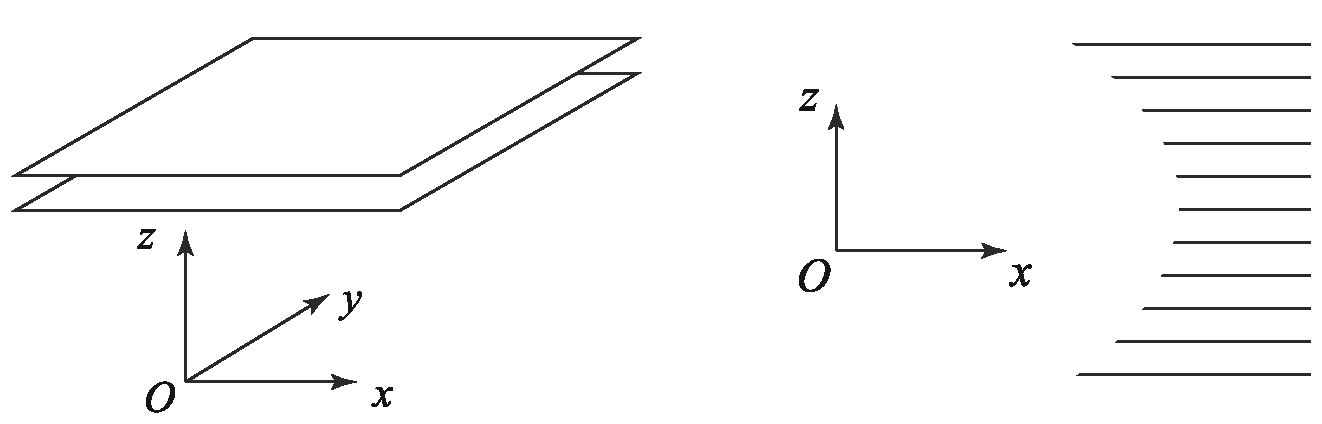
\includegraphics[width = 0.7\textwidth]{images/em-theory-6.pdf} 
\end{center}

\tagged{student}{\vspace*{4cm}}
\begin{taggedblock}{teacher}
\noindent
解析:1. 根据电磁场边界条件,$z=0$和$z=d$处的电场强度为零,相位取$0$或$\pi$:
\[\Delta \varphi = \frac{2\pi d}{\lambda_z}-\frac{2\pi \cdot 0}{\lambda_z}=m\pi\]
即:
\[\lambda_z=\frac{2d}{m}\]
2. \[\lambda_z=2d\]
3. \[z^2 = 4L \cdot (-x)\]
\end{taggedblock}
\end{example}
%%%%%%%%%%%%%%%%%%%%%%

\section{光的电磁理论}
\begin{figure}[htb]
\centering
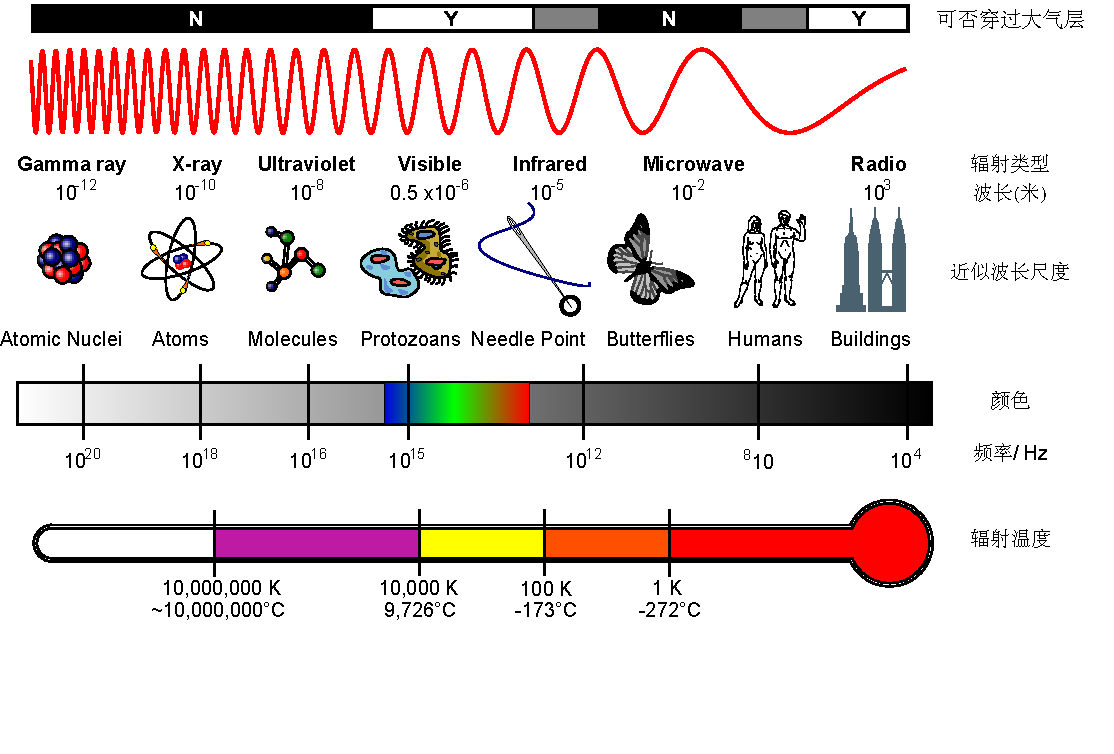
\includegraphics[width=0.9\textwidth]{images/em-theory-3.pdf}
\caption{电磁波谱}
\label{fig: em-theory-3}
\end{figure}
当意识到光是电磁波的一种时,就有了理解光学现象更多的方法,并且能够在更多的物理量之间建立联系。
以下就是一些基于光的电磁理论得到的一些结论:
\begin{description}
\item[{\heiti 光的颜色}] 可见光的颜色由电磁波的波长所决定,一般人的眼睛可以感知波长在$400-760\unit{nm}$的电磁波\footnote{极个别的人能够感知到$380-780\unit{nm}$范围的电磁波。},其中红光对应的波长较长,紫光对应的波长较短,正常视力的人眼对波长约为$555\unit{nm}$的绿光最为敏感。
波长比红光长的电磁波随着波长的增加称为{\heiti 红外线}(infrared, IR)、{\heiti 微波}(microwave)、{\heiti 射电}(radio wave)等,而随着波长的减小,超出可见光范围的电磁波则被称为{\heiti 紫外线}(ultraviolet, UV)、{\heiti X射线}(X ray)以及{\heiti $\gamma$射线}($\gamma$ ray)。
不同波长的电磁波在传播时有不同的特点。

\item[{\heiti 折射率}] 当光在相对介电常数为$\varepsilon_r$,相对磁导率为$\mu_r$的透明介质中传播时,由于光和物质的相互作用,介质中的光速由
\begin{equation}
v^2 = \frac{1}{\varepsilon\mu} = \frac{c^2}{\varepsilon_r\mu_r}
\end{equation}
给出,对于普通的电介质$\mu_r\approx 1$,可得$v = \frac{c}{\sqrt{\varepsilon_r}}$,可知介质的折射率
\begin{equation}
n = \sqrt{\varepsilon_r}
\end{equation}
对于透明介质折射率的测量验证了这一结果,另外它也是光的电磁理论正确的一个实验依据,因为折射率和介电常数在过去认为是两个无关的物理量,只有光的电磁理论才能够将两者联系起来。

\item[{\heiti 反射光和透射光的强度}]
传统的几何光学中光在透明介质表面即可能反射,也可能折射,它们分别满足简单的反射、折射定律,但没有给出反射光和折射光的强度关系。
我们知道做为电磁波,光的能量正比于振幅的平方,而借助光的电磁理论以及光和介质的相互作用的特点可以帮助我们从理论上给出反射光和折射光振幅的关系,也就进一步得到了反射、折射光强度的关系。
在最简单的情况下当光从折射率$n_1$介质垂直入射到折射率$n_2$介质时,界面上产生反射和透射射,这时反射光和透射光的强度与介质的折射率有关,设入射光的电场强度为$E_0$,反射和透射光的电场强度分别为$E_1$和$E_2$,理论计算表明:
\begin{equation}\label{eqn: em-wave-反射率}
\frac{E_1}{E_0} = \frac{n_1-n_2}{n_1+n_2},\qquad \frac{E_2}{E_0} = \frac{2n_1}{n_1+n_2},\qquad \text{反射率} = \Bigg|\frac{E_1}{E_0}\Bigg|^2
\end{equation}

\item[{\heiti 色散关系}]
不同频率的光在给定的介质中的折射率不尽可同,物理上将角频率$\omega$随波数$k$的函数关系$\omega(k)$称为{\heiti 色散关系}(dispersion relation)。
若无光的电磁理论,色散关系只能够依靠实验测量,但在光的电磁理论基础上,当细致地研究了光是如何与介质分子、原子相互作用的规律后理论上可以计算出色散关系。历史上洛伦兹(\textit{H. A. Lorentz})在这方面做出了开创性的工作。
\end{description}



